\documentclass[12pt]{report}
\usepackage[utf8]{inputenc}
\usepackage[spanish,es-noshorthands]{babel}
\addto\captionsspanish{%
    \renewcommand{\listfigurename}{Índice de gráficas}%
}
\usepackage{amsmath}
\usepackage{siunitx}
\sisetup{
    per-mode=symbol,
    range-phrase={--},
    range-units=single
}
\DeclareSIUnit{\dBm}{dBm}
\DeclareSIUnit{\sample}{Sa}
\usepackage{longtable,booktabs,array,tabularx}
\usepackage{graphicx}
\usepackage{hyperref}
\usepackage[spanish]{cleveref}
\usepackage[backend=biber,style=apa]{biblatex}
\addbibresource{refs.bib}
\newcolumntype{P}[1]{>{\raggedright\arraybackslash}p{#1}}
\newcolumntype{Y}{>{\raggedright\arraybackslash}X}
\newcommand{\notafigura}[1]{%
    \par\medskip
    {\raggedright\footnotesize\textit{Nota.} #1\par}%
}
\begin{document}
\begin{center}
UNIVERSIDAD DE EJEMPLO\\
FACULTAD DE PRUEBAS
\end{center}
\clearpage
\tableofcontents
\listoftables
\listoffigures
\clearpage

\chapter{Primero}\label{chap:uno}
\section{Alfa}\label{sec:alfa}
\subsection{Beta}\label{subsec:beta}
\subsubsection{Gamma}
\label{subsubsec:gamma}
\label{subsubsec:gamma-alias}
Ver \cref{subsubsec:gamma}, \cref{subsubsec:gamma-alias} y \cref{sec:alfa,subsec:beta}.
Ecuaciones \cref{eq:uno,eq:dos}. \Cref{tab:larga} resume; el \cref{tab:ancha} y la \cref{fig:dibujo}.
Potencia de \SI{5}{\dBm} a \SI{10}{\giga\sample\per\second}, \SIrange{300}{900}{\mega\hertz},
\SI{-3}{\decibel} y \SI{10}{\percent} de margen. En forma $P_{1\,\mathrm{dB}}>\SI{10}{\dBm}$.
Según \textcite{autora2020} y otros \parencite{autora2020}.
\newpage
Texto tras el salto de página.
\begin{equation}a=b\label{eq:uno}\end{equation}
\begin{equation}c=d\label{eq:dos}\end{equation}
\begin{longtable}{@{}P{2cm}p{4cm}@{}}
\caption{Una tabla larga}\label{tab:larga}\\
\toprule
Nodo & Etapa\\
\midrule
\endfirsthead
\toprule
Nodo (cont.) & Etapa (cont.)\\
\midrule
\endhead
\midrule
\multicolumn{2}{r}{Continúa en la página siguiente}\\
\endfoot
\bottomrule
\multicolumn{2}{@{}p{\textwidth}@{}}{%
    \vspace{4pt}\footnotesize\textit{Nota.} Nota final de la tabla larga.}\\
\endlastfoot
FILTER\_OUT & Filtro\\
\end{longtable}
\begin{table}[h]
\caption{Tabla ancha}\label{tab:ancha}
\begin{tabularx}{\textwidth}{@{}P{3cm}YY@{}}
\toprule
a & b & c\\
\bottomrule
\end{tabularx}
\end{table}
\begin{figure}[h]
\centering
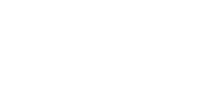
\includegraphics[width=0.5\textwidth]{dibujo.svg}
\caption{Un dibujo}\label{fig:dibujo}
\notafigura{Elaboración propia con datos de prueba.}
\end{figure}
\addcontentsline{toc}{chapter}{Entrada manual}

{\sloppy
\printbibliography[heading=bibintoc, title={Referencias del documento}]
}

\appendix
\crefalias{chapter}{appendix}
\chapter{Detalles}\label{anx:detalles}
Ver \cref{anx:detalles}, \cref{anxsec:uno}, \cref{eq:anexo} y \Cref{tab:anexo}.
\section{Uno del anexo}\label{anxsec:uno}
Texto.
\begin{equation}y=2\label{eq:anexo}\end{equation}
\begin{table}[h]
\caption{Tabla del anexo}\label{tab:anexo}
\begin{tabular}{ll}
x & y\\
\end{tabular}
\end{table}
\end{document}
